\section{Semaine 9 : 03/04/2023 - 07/04/2023}
\graphicspath{{semaines/semaine_9/images/}}

\begin{abstract}
	Après les résultats obtenus avec le FNO, on va essayer de comparer les temps d'exécution et les erreurs obtenus pour FEM, Phi-FEM, le FNO et le FNO+corr à différentes époques.
	
	Après discussion avec Emmanuel, on va considérer une level-set du type $\tilde{\phi}=u_{ex}+\epsilon*P$. On va tester le rehaussement avec FEM puis avec PhiFEM pour différents $m$ sur cette solution perturbée.
	
	(Vendredi est férié)
\end{abstract}

\subsection{Temps d'exécution (avec FNO)}

On considère, comme pour les boxplots de la semaine dernière, $f$ gaussienne :
$$f(x,y) = \exp\left(-\frac{(x-\mu_0)^2 + (y-\mu_1)^2}{2\sigma^2}\right)\,, $$ 
avec $\sigma \sim \mathcal{U}([0.1,0.6])$ et $\mu_0, \mu_1 \sim \mathcal{U}([0.5-\sqrt{2}/4, 0.5+\sqrt{2}/4])$ à condition que $\phi(\mu_0, \mu_1) < -0.05$. \\

Voici les résultats obtenus :

\begin{minipage}{\linewidth}
	\centering
	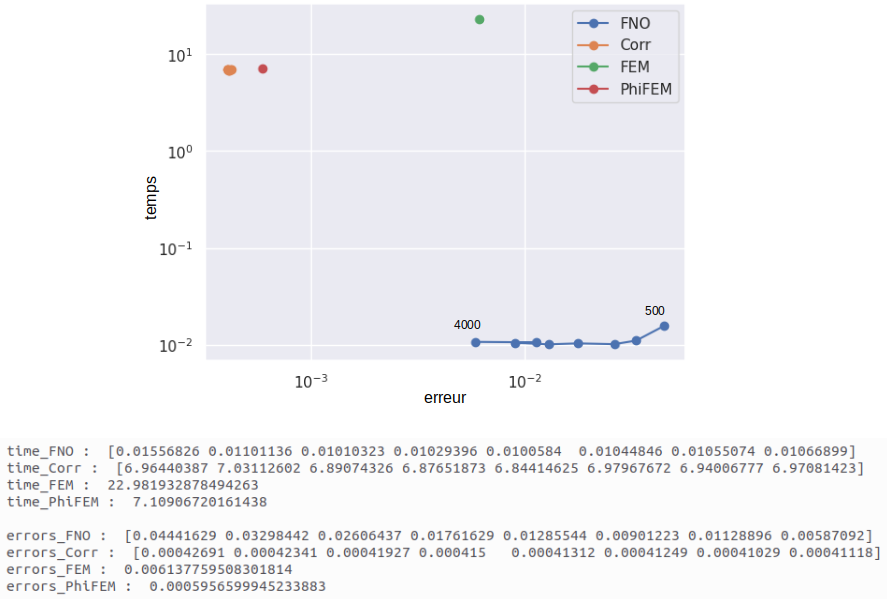
\includegraphics[width=\linewidth]{time_FNO.png}
\end{minipage}

\subsection{Rehaussement avec FEM}

On se place sur le carré $[0,1]^2$. 

On souhaite résoudre le problème de Poisson avec condition de Dirichlet non homogène :

$$\left\{\begin{aligned}
	&-\Delta u=f \quad &&\Omega \\
	&u=g \quad &&\Gamma
\end{aligned}\right.$$

On considère la solution analytique suivante :
$$u_{ex}(x,y) = S\times\sin(2\pi fx + \varphi)\times\sin(2\pi fy + \varphi)$$ 

$S$ est l'amplitude du signal, $f$ la fréquence du signal et $\varphi$ la phase à l'origine.

On pose alors
$$f(x,y)=8\pi^2 Sf^2\times\sin(2\pi fx + \varphi)\times\sin(2\pi fy + \varphi), \quad g(x,y)=u_{ex}(x,y)$$

On considère qu'après une utilisation du FNO, on obtient une solution du type
$$u_p = u_{ex}+\epsilon P(x,y)$$

avec $\epsilon$ petit et $P$ la perturbation définie par
$$P(x,y)=S_p\times\sin(2\pi f_px + \varphi_p)\times\sin(2\pi f_py + \varphi_p)$$

On considère alors la solution rehaussée par $m$ :
$$\tilde{\phi}=u_p+m$$

avec $m$ une constante.

Voici la solution pour $S=0.5$, $f=1$, $\varphi=0$ et $m=1$ (à gauche la solution $u$ en 2d, au milieu la solution $u$ en 3D et à droite la solution exacte rehaussée $u+m$ en 3D) :

\begin{minipage}{\linewidth}
	\centering
	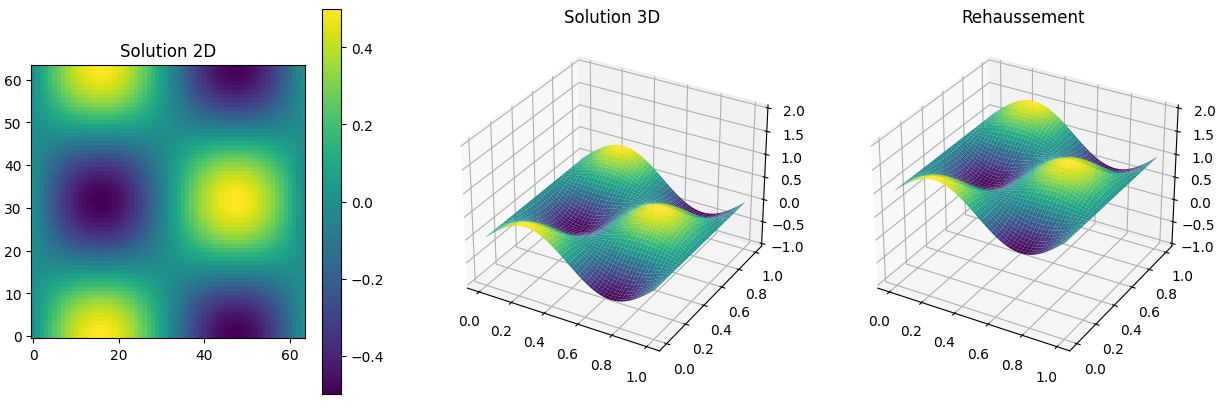
\includegraphics[width=0.8\linewidth]{solution.png}
\end{minipage}

On se ramène alors on problème
$$\left\{\begin{aligned}
	&-\Delta (u_pC)=f \quad &&\Omega \\
	&C=1 \quad &&\Gamma
\end{aligned}\right.$$

Et donc
$$\left\{\begin{aligned}
	&-\Delta(\tilde{\phi}C)=f \quad &&\Omega \\
	&C=1 \quad &&\Gamma
\end{aligned}\right.$$

On obtient alors
$$\tilde{u}=\tilde{\phi}C$$

Et donc
$$u_C=\tilde{\phi}C-m$$

On obtient alors la formulation variationnelle suivante (avec comme fonction test $\tilde{\phi}v$) :
$$\int_{\Omega}\nabla (\tilde{\phi}C)\cdot\nabla (\tilde{\phi}v)=\int_\Omega f\tilde{\phi}v$$

\begin{Rem}
	Attention $u$ et $u_p$ doivent avoir les mêmes conditions aux bords donc $P$ doit être nulle au bord. On prendra 10 comme degré de quadrature et 10 comme degré d'intepolation.
\end{Rem}

\subsubsection*{Test 1 : $g=0$}

On prend $S,S_p=0.5$, $\epsilon=10^{-3}$ et $\varphi,\varphi_p=0$. Ainsi $g=0$ sur $\Gamma$. 

Voici les résultats obtenus en faisant varier $f$, $f_p$ et $m$ (à gauche les erreurs en norme $L^2$, à droite les facteurs avec FEM) :

\begin{minipage}{\linewidth}
	\centering
	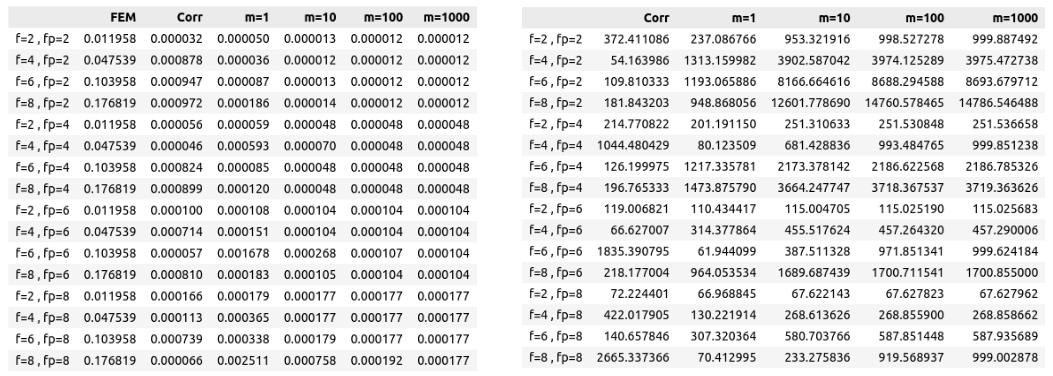
\includegraphics[width=0.9\linewidth]{test1.png}
\end{minipage}

On prend toujours $S,S_p=0.5$, $\varphi,\varphi_p=0$. On fixe cette fois-ci $f=8$ et $f_p=3$ et on prend $\epsilon=10^{-4}$. 

On obtient les résultats suivants :

\begin{minipage}{\linewidth}
	\centering
	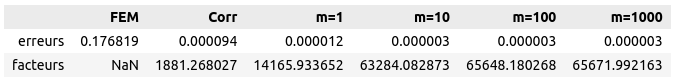
\includegraphics[width=0.6\linewidth]{test1_bis.png}
\end{minipage}

\begin{Rem}
	On a le même type de résultat avec $S=1$ et $S_p=0.25$.
\end{Rem}

\subsubsection*{Test 2 : $g\ne 0$}

On prend $S,S_p=0.5$, $\epsilon=10^{-3}$, $\varphi=0.25$ et $\varphi_p=0$.

Voici les résultats obtenus en faisant varier $f$, $f_p$ et $m$ (à gauche les erreurs en norme $L^2$, à droite les facteurs avec FEM) :


\begin{minipage}{\linewidth}
	\centering
	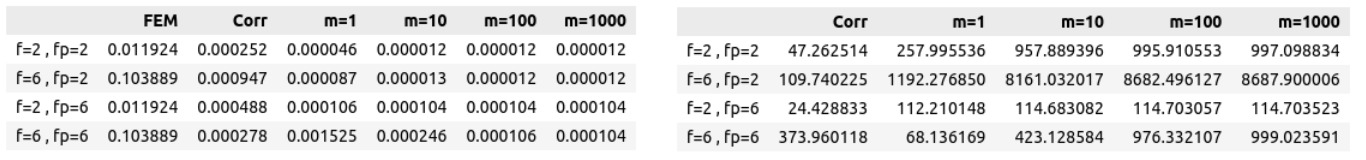
\includegraphics[width=\linewidth]{test2.png}
\end{minipage}

\subsection{Rehaussement avec PhiFEM}

On souhaite effectuer le même type de tests avec PhiFEM.

On se place encore sur le carré $[0,1]^2$. On prend alors
$$\phi (x,y)=||x-0.5||_\infty-0.5$$

On considérera le domaine environnant $\mathcal{O}=[-0.5,1.5]^2$.

On considère encore la solution analytique suivante :
$$u_{ex}(x,y) = S\times\sin(2\pi fx + \varphi)\times\sin(2\pi fy + \varphi)$$ 

et pour $p=0$, $g(x,y)=0$.

De la même manière que pour FEM, on va considérer la solution rehaussée par $m$ :
$$\tilde{\phi}=u_p+m$$

\subsubsection*{Test}

Comme pour le Test 1 de FEM, on prend $S,S_p=0.5$, $\epsilon=10^{-2}$ et $\varphi,\varphi_p=0$. Ainsi $g=0$ sur $\Gamma$. 

Voici les résultats obtenus en faisant varier $f$, $f_p$ et $m$ (à gauche les erreurs en norme $L^2$, à droite les facteurs avec PhiFEM) :

\begin{minipage}{\linewidth}
	\centering
	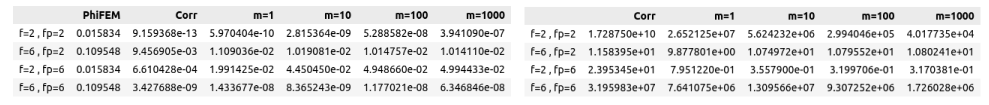
\includegraphics[width=\linewidth]{test_phifem.png}
\end{minipage}

\conclusion{Il semblerait qu'il y ait un problème avec PhiFEM. On va donc de nouveau mettre le FNO de côté.}